\documentclass{article}
\usepackage[utf8]{inputenc}
\usepackage{graphicx}
\usepackage{listings}
\title{Information System - Lab work 6}
\author{Tran Thi Hong Hanh}
\date{10 November 2017}

\begin{document}

\maketitle
\section*{Database}
\begin{itemize}
	\item employees (emp\_no, birth\_date, first\_name, last\_name, gender)
	\item departments (dept\_no, dept\_name)
	\item dept\_emp (emp\_no, dept\_no, from\_date, to\_date)
	\item dept\_manager (dept\_no, emp\_no, from\_date, to\_date)
	\item titles (emp\_no, title, from\_date, to\_date)
	\item salaries (emp\_no, salary, from\_date, to\_date)
\end{itemize}
\section*{SQL queries using subqueries}
\begin{enumerate}
	\item Who have the same name as the managers of the "Finance" department?\\
	\begin{lstlisting}{showstringspaces=false}[language=SQL]
SELECT emp_no, CONCAT(first_name, "", last_name) AS full_name 
FROM employees WHERE last_name IN (
	SELECT last_name 
    FROM dept_manager 
    JOIN employees ON dept_manager.emp_no = employees.emp_no
    JOIN departments ON dept_manager.dept_no = departments.dept_no
	WHERE dept_name = "finance");
	\end{lstlisting}
	
	\item Who in the "Production" department were hired after the promotion of the last manager in that departments?\\
	\begin{lstlisting}{showstringspaces=false}
SELECT employees.emp_no,
CONCAT(first_name, "", last_name) AS fullname, hire_date
FROM employees 
JOIN (SELECT emp_no FROM departments 
	  NATURAL JOIN dept_emp
	  WHERE dept_name = 'Production') AS subquery1
	  ON employees.emp_no = subquery1.emp_no
	  WHERE hire_date > (SELECT MAX(from_date)
	  		FROM dept_manager 
	  		NATURAL JOIN departments
			WHERE dept_name = 'Production');
	\end{lstlisting}
	
	
	\item Find the average salary of each department, from highest to lowest.	
	\begin{lstlisting}{showstringspaces=false}
SELECT dept_no, AVG(salary)
FROM (SELECT salary, dept_no 
	  FROM salaries JOIN dept_emp 
	  ON dept_emp.emp_no = salaries.emp_no) AS subquery
GROUP BY dept_no
ORDER BY AVG(salary) DESC;

	\end{lstlisting}
	
	\item Find the average salary for each type of Engineer, from highest to lowest.
	
	\begin{lstlisting}{showstringspaces=false}
SELECT * FROM (SELECT title, salary FROM titles
	JOIN salaries ON salaries.emp_no = titles.emp_no
	WHERE title LIKE '%Engineer%') AS subquery
GROUP BY title
ORDER BY AVG(salary) DESC;
	\end{lstlisting}
		
\end{enumerate}

\section*{Results}

The figure below presents the results after implement queries (limit from 0 to 10 for some long results
) above:\\
\begin{figure}
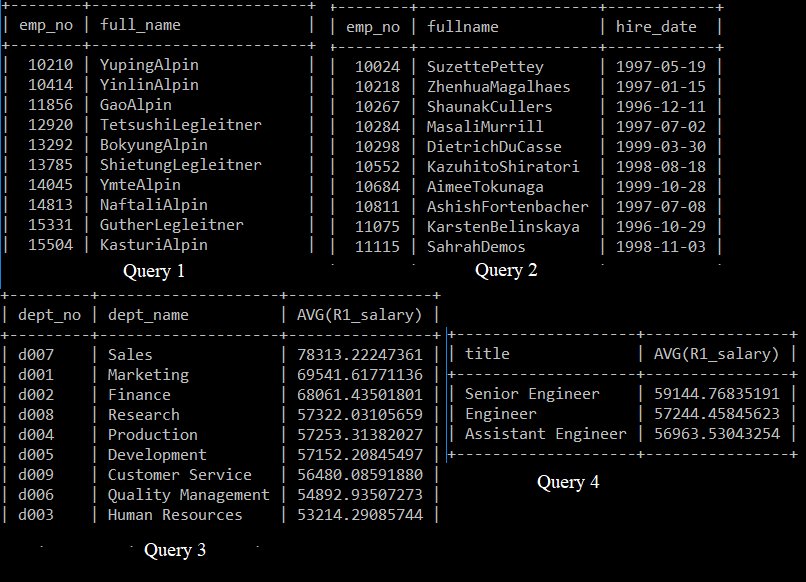
\includegraphics[scale = 0.9]{result.PNG}
\caption{Results}
\end{figure}
\end{document}
